
\AtBeginSection[]
{
  \begin{frame}{Let the System Learn a Game}
  \begin{columns}[t]
  \begin{column}{5cm}
  \tableofcontents[sections={1-3},currentsection,hideothersubsections]
  \end{column}
  \begin{column}{5cm}
  \tableofcontents[sections={4-6},currentsection,hideothersubsections]
  \end{column}
  \end{columns}
  \end{frame}
}

\begin{frame}
\titlepage
\end{frame}

\begin{frame}{Let the System Learn a Game}
  \begin{columns}[t]
  \begin{column}{5cm}
  \tableofcontents[sections={1-3},hideallsubsections]
  \end{column}
  \begin{column}{5cm}
  \tableofcontents[sections={4-6},hideallsubsections]
  \end{column}
  \end{columns}

\end{frame}

\section{Introduction}
\subsection{Rappel historique}
%----------------------------------------
% RAPPEL HISTORIQUE - DEEP BLUE
%----------------------------------------

\begin{frame}{Rappel historique}{Deep Blue}

\begin{block}{Deep Blue} 
\begin{itemize}
\item Victoire contre Garry Kasparov en 1997.
\item $1^{\grave{e}re}$ défaite de grand maître sous contraintes normales de temps.
\end{itemize}
\end{block}

\pause

\begin{block}{R. Levinson} 
\begin{itemize}
\item \textit{\og But doesn't know that it's playing chess.\fg{}}
\item Intelligence? Artificielle? Synthétique?
\end{itemize}
\end{block}

\end{frame}



%----------------------------------------
% RAPPEL HISTORIQUE - THÉORIE DES JEUX
%----------------------------------------

\begin{frame}{Rappel historique}{Théorie des Jeux}

\begin{block}{Théorème du Minimax} 
\begin{itemize}
\item J. Von Neumann, 1928.
\item \textit{Stratégie optimale pour un joueur donné.}
\end{itemize}
\end{block}

\pause

\begin{block}{Équilibre de Nash} 
\begin{itemize}
\item J. F. Nash, 1950.
\item \textit{Union de stratégies, localement optimale pour tous.}
\end{itemize}
\end{block}

\end{frame}


%----------------------------------------
% RAPPEL HISTORIQUE - LIMITES
%----------------------------------------

\begin{frame}{Rappel historique}{Limites}

\begin{block}{Domaine d'application}
\begin{itemize}
\item \underline{Minimax}: Jeux compétitifs, à deux joueurs, à somme nulle.
\item \underline{Minimax \& Nash}: Durée et nombre d'options finis.
\end{itemize}
\end{block}

\pause

\begin{block}{Temps de calcul}
\begin{itemize}
\item Complexité moyenne \emph{$O(b^{\frac{d}{2}})$} si trié et élagé:
	\begin{itemize}
	\item d : longeur de la partie.
	\item b : nombre d'options par tour.
	\end{itemize}
\item En pratique: besoin d'heuristiques, donc perte d'optimalité.
\end{itemize}
\end{block}

\end{frame}

\subsection{Projet de recherche}
\begin{frame}{Présentation du sujet}
	\begin{itemize}
		\item Intelligence artificielle
		\pause
		\item Approche différente d'un projet
		\pause
		\item Rêve de l'IA
	\end{itemize}
\end{frame}

\begin{frame}{Présentation du sujet}{Une approche cognitive}
	\begin{itemize}
		\item Apprentissage
		\item Reconnaissance de formes
		\item Classification
		\item Polyvalence du système
	\end{itemize}
\end{frame}


\subsection{Un modèle de conscience artificielle}
\begin{frame}{Un modèle de conscience artificielle}{Origine du modèle}
\begin{itemize}
  \item ``Consicence
  artificielle'' par Guillaume Tisserant, Guillaume Travail du module
  'Cognition' du M2 en 2010
  \item Modèle de représentation proposé dans le Chapitre 4.
\end{itemize}
\end{frame}

\begin{frame}{Un modèle de conscience artificielle}{Version simplifiée du
modèle}
\begin{center}
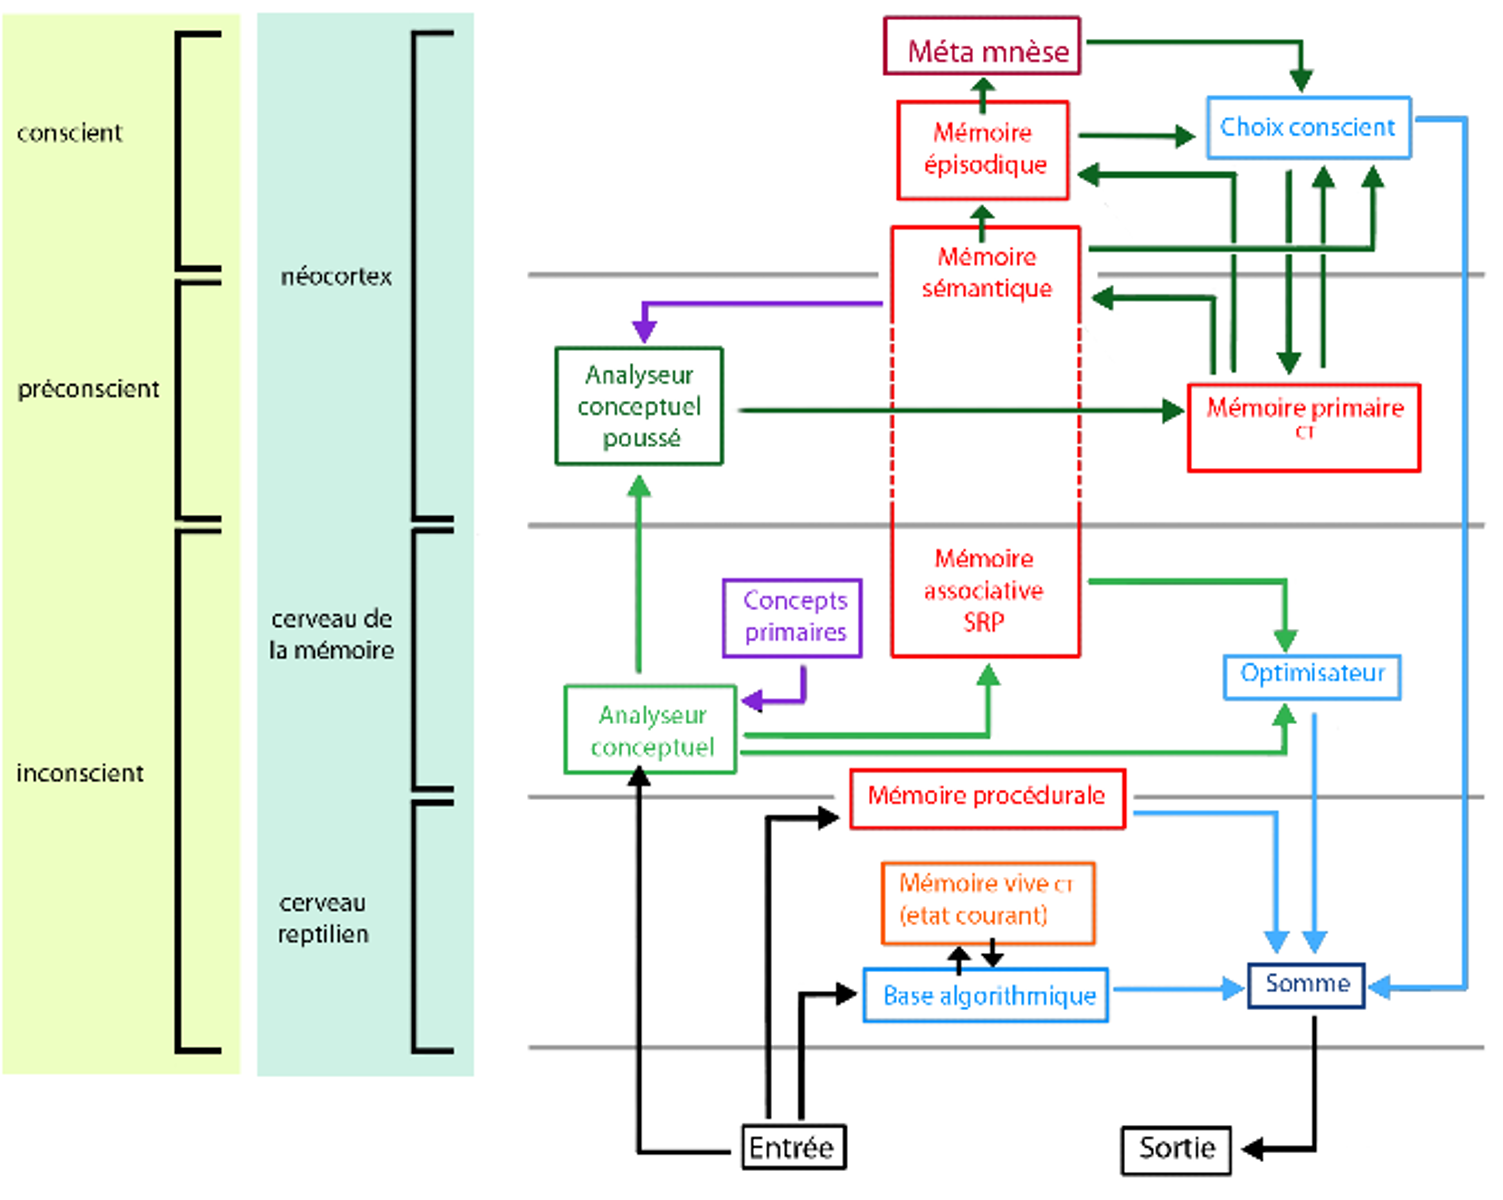
\includegraphics[width=0.9\textwidth]{img/intro/modele_original}
\end{center}
\end{frame}



\section{Application: game modeling}
%--------------------------------------------------------------------------------
% FIELD ADVANTAGES
%--------------------------------------------------------------------------------
\begin{frame}{Application: game modeling}{Field advantages}
\end{frame}

%--------------------------------------------------------------------------------
% CHOSEN GAME: "REVERSI"
%--------------------------------------------------------------------------------
\begin{frame}{Application: game modeling}{Chosen game: "Reversi"}
\end{frame}

%--------------------------------------------------------------------------------
% VON NEUMANN'S THEOREM
%--------------------------------------------------------------------------------
\begin{frame}{Application: game modeling}{Von Neumann's theorem}
\end{frame}

%--------------------------------------------------------------------------------
% DRAWBACKS OF MINIMAX
%--------------------------------------------------------------------------------
\begin{frame}{Application: game modeling}{Drawbacks of Minimax}
\end{frame}

%--------------------------------------------------------------------------------
% AN ALTERNATIVE
%--------------------------------------------------------------------------------
\begin{frame}{Application: game modeling}{An alternative}
\end{frame}

\section{"Cogito" system overview}
%-------------------------------------------------------------------------------
% BOARD ENCODING
%-------------------------------------------------------------------------------
\subsection{Board encoding}
\begin{frame}{``Cogito" system overview}{Board encoding}

Each encountered state of the board is an object, while certain configurations 
deemed are attributes. A configuration is invariant with regards to translations 
and rotations.

\end{frame}

%-------------------------------------------------------------------------------
% EVALUATING CONFIGURATIONS
%-------------------------------------------------------------------------------
\subsection{Evaluating configurations}
\begin{frame}{``Cogito" system overview}{Evaluating configurations}

When the game ends the final configuration is given a value based on whether the 
agent has won or last. This value and is propagated backwards through previous
board states with linear attenuation. The value of a state board the value 
of its configurations.

\end{frame}

%-------------------------------------------------------------------------------
% GENERATING NEW CONFIGURATIONS
%-------------------------------------------------------------------------------
\subsection{Generating new configurations}
\begin{frame}{``Cogito" system overview}{Generating new configurations}

New relevant configurations are deduced by attempting to locally extend an 
existing configuration shared by two or more winning or losing board states.

\end{frame}

%-------------------------------------------------------------------------------
% PUTTING IT ALL TOGETHER
%-------------------------------------------------------------------------------
\subsection{Putting it all together}
\begin{frame}{``Cogito" system overview}{Putting it all together}

The system receives a set of possible moves to choose from. By evaluating each 
resulting board state based on prior experience it is able to choose the one 
which seems most beneficial.

Nota Bene: there is no look-ahead, but as we are essentially engineering a 
dynamic heuristic the system could be easily combined with a limited-depth 
Minimax implementation.

\end{frame}

\section{What FCA brings to the table}
%-------------------------------------------------------------------------------
% ELIMINATIONS OF REDUNDANCY
%-------------------------------------------------------------------------------
\subsection{Reducing redundancy}
\begin{frame}{What FCA brings to the table}{Reducing redundancy}

\begin{itemize}
\item Attributes always found together can be merged,
\item<2-> beware of introducing errors!
\end{itemize}

\begin{figure}[ht]
  \begin{minipage}[t]{0.3\linewidth}
    \vspace{0pt}
    \centering
    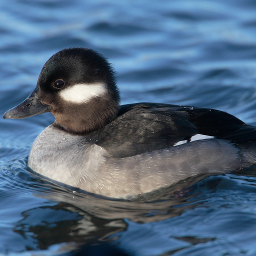
\includegraphics[width=\textwidth]{img/fca/duck1}
    \\ \color{green}{\footnotesize $hasBill(x) \wedge isDuck(x)$}
  \end{minipage}
  \hfill
  \begin{minipage}[t]{0.3\linewidth}
    \vspace{0pt}
    \centering
    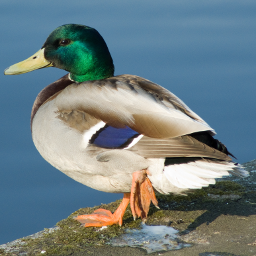
\includegraphics[width=\textwidth]{img/fca/duck2}
    \\ \color{green}{\footnotesize $hasBill(y) \wedge isDuck(y)$}
  \end{minipage}
  \hfill
  \pause
  \begin{minipage}[t]{0.3\linewidth}
    \vspace{0pt}
    \centering
    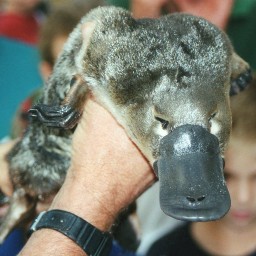
\includegraphics[width=\textwidth]{img/fca/platypus}
    \\ \color{red}{\footnotesize $hasBill(z) \wedge \neg{}isDuck(z)$}
  \end{minipage}
\end{figure}

\end{frame}

%-------------------------------------------------------------------------------
% FASTER QUERIES
%
%% on peut en dégager une hiérarchie des RPBS. Celle-ci pourrait
%% permettre une recherche plus intelligente des RPBS (réduction du
%% nombre d'homomorphismes à appliquer sur chaque plateau) et donc un
%% gain de temps pour la prise de décision sans devoir réduire
%% drastiquement le nombre de RPBS. On peut imaginer que le système
%% effectuerait une recherche approfondie à posteriori afin de ne pas
%% biaiser l'apprentissage. (L'idée générale est, pendant la phase de
%% jeu, de classer le CBS à évaluer dans un concept et de lui
%% attribuer le point associé à celui-ci. Ce qui permettrait de
%% profiter de la structure du treillis pour diminuer drastiquement le
%% nombre de RPBS rechercher. À savoir que c'est l'étape la plus
%% coûteuse.)
%-------------------------------------------------------------------------------
\subsection{Faster queries}
\begin{frame}{What FCA brings to the table}{Faster queries}


  \begin{itemize}
    \item Le treillis de FCA nous offre un ordre partiel sur les
      configurations de plateau
    \item Il est possible de ce servir de cette ordre pour effectuer
      une exploration partiel des configurations lors de l'analyse
      d'un plateau
    \item toutefois pour ne pas biaiser cette ordre partiel il est
      important d'effectuer une recherche complète a posteriori
    
  \end{itemize}



\end{frame}

%-------------------------------------------------------------------------------
% CHOOSING NEW CONFIGURATIONS 
%
%% Les RPBS introduit dans des concepts
%% parents d'un concept commun (introduisant au moins un CBS), ont
%% potentiellement une sous-partie commune qu'il peut-être intéressant
%% d'extraire comme un nouveau RPBS. (voir common_part.png)
% -------------------------------------------------------------------------------
\subsection{Discovering new configurations}
\begin{frame}{What FCA brings to the table}{Discovering new
    configurations}

\begin{minipage}[t]{0.40\linewidth}
  \begin{figure}[ht]
    \centering
    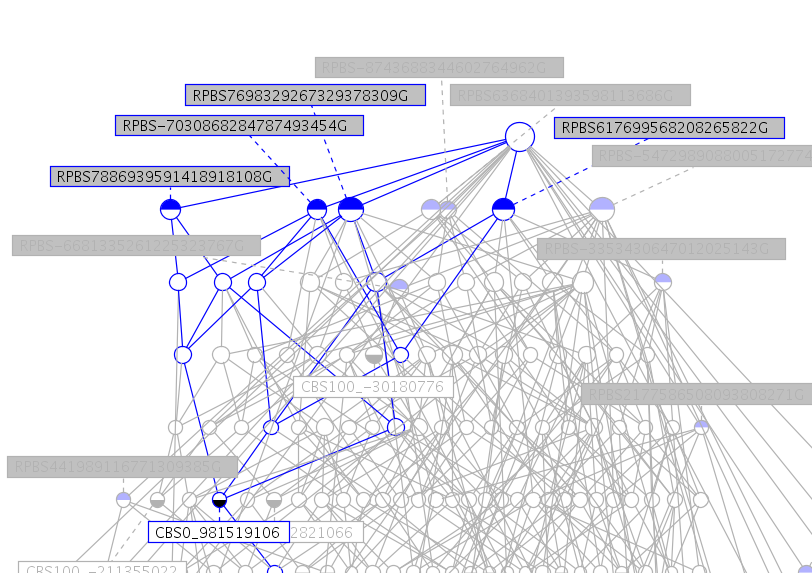
\includegraphics[width=\textwidth]{img/fca/common_part}
  \end{figure}
\end{minipage}
\begin{minipage}{0.60\linewidth}
  \begin{itemize}
    \item 
  \end{itemize}
\end{minipage}

\end{frame}


% ADDED INSIGHT
%-------------------------------------------------------------------------------
\subsection{Added insight}
\begin{frame}{What FCA brings to the table}{Added insight}

\begin{minipage}[t]{0.40\linewidth}
  \begin{figure}[ht]
    \centering
    %\includegraphics[width=\textwidth]{}
  \end{figure}
\end{minipage}
\begin{minipage}{0.60\linewidth}
  \begin{itemize}
    \item 
  \end{itemize}
\end{minipage}

\end{frame}

\section{Discussion}
\begin{frame}{Conclusion and discussion}

\centering \LARGE Thank you for your time. \\ Are there any questions?

\end{frame}